\section{V13}
\subsection{Kommunikation zwischen Rechnersystemen}
F"ur eine rechner"ubergreifende Kommunikation stehen heutzutage verschiedene Protokolle und Spezifikationen zur Verf"ugung. Trotz der Vielfalt basieren heute die meisten Implementationen auf den Grundkonzepten des OSI-Referenzmodells und legen damit schon die entscheidenden Weichen f"ur geordnete Kommunikationsabl"aufe und saubere Netzwerkstrukturen.

\begin{minipage}{9cm}
\subsubsection{ISO/OSI-Modell}
	Das OSI-Referenzmodell beschreibt modellhaft die Kommunikation in \textbf{7}
 hierarchischen Schichten (Layer) unterschiedlicher Abstraktion. Hierbei stellt eine Schichht \textbf{i} Dienstleistungen f"ur die dar"Uber liegende Schicht \textbf{i+1} zur Verf"ugung, sie selbst bezieht Dienstleistungen von der unter ihr liegende Schicht \textbf{i-1}.
\end{minipage}
%
\begin{minipage}{0.5cm}
	\-\
\end{minipage}
%
\begin{minipage}{9cm}
	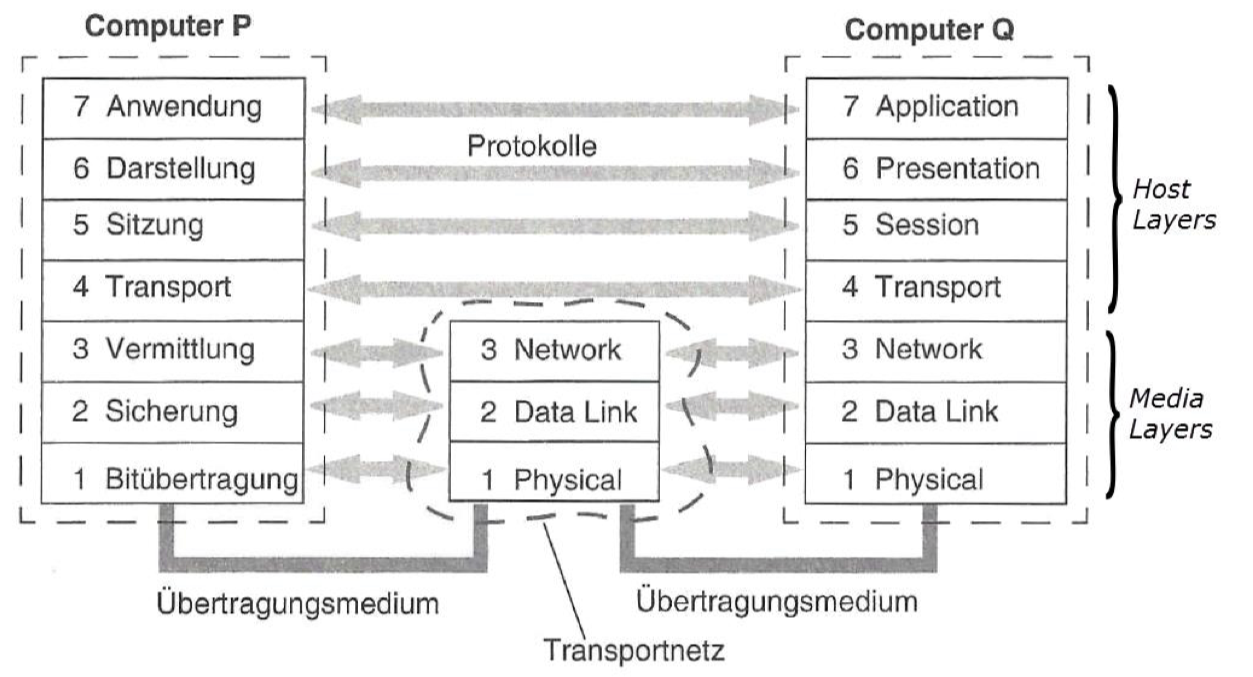
\includegraphics[width=8cm]{images/OSI-Referenzmodell}
\end{minipage}

 Das OSI-Referenzmodell stellt eine Konstruktionsanleitung f"ur Netzwerksoftware da. "Uber insgesamt sieben Layer sind abstrakte Funktionen definiert, die aufeinander aufbauen. Beim Datentransport werden die Nutzdaten in den jeweiligen Protokollrahmen eingebettet und der unteren Schicht weiter gereicht. $\Rightarrow$ Kapselung\\

 \begin{minipage}{10.5cm}
 	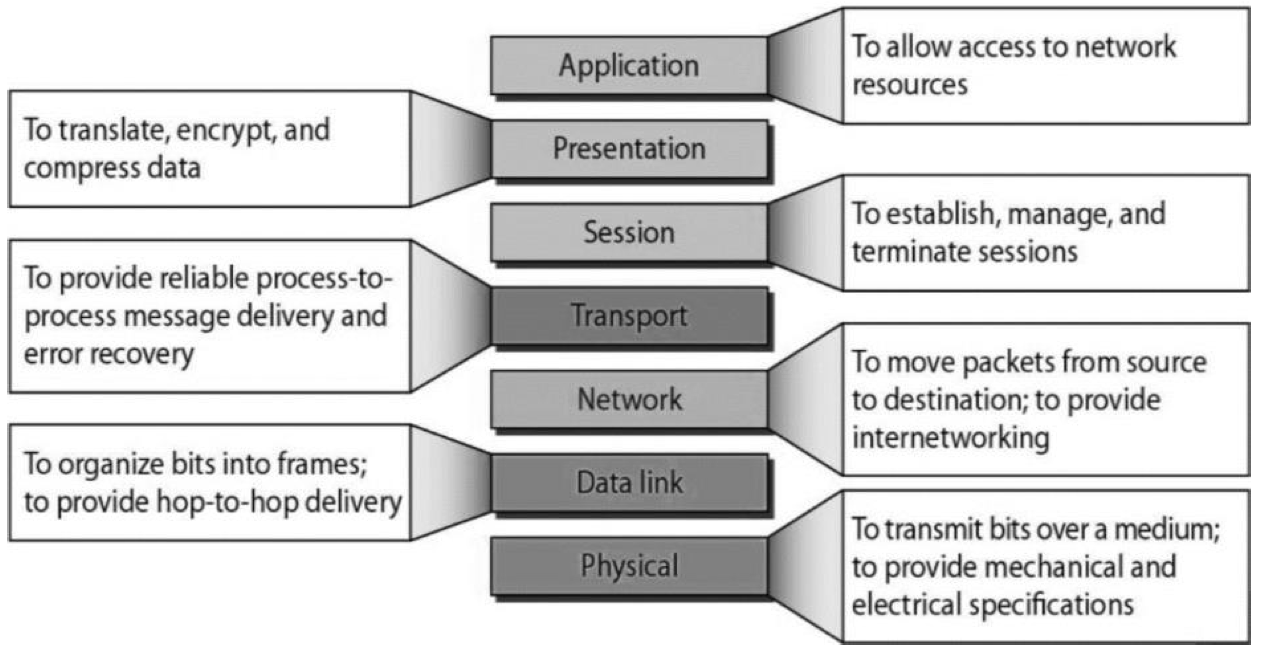
\includegraphics[width=10 cm]{images/OSI-Layer}
 \end{minipage}
 %
 \begin{minipage}{0.5cm}
 	\-\
 \end{minipage}
 %
 \begin{minipage}{7.5cm}
 	\textbf{Kapselung}\\
 	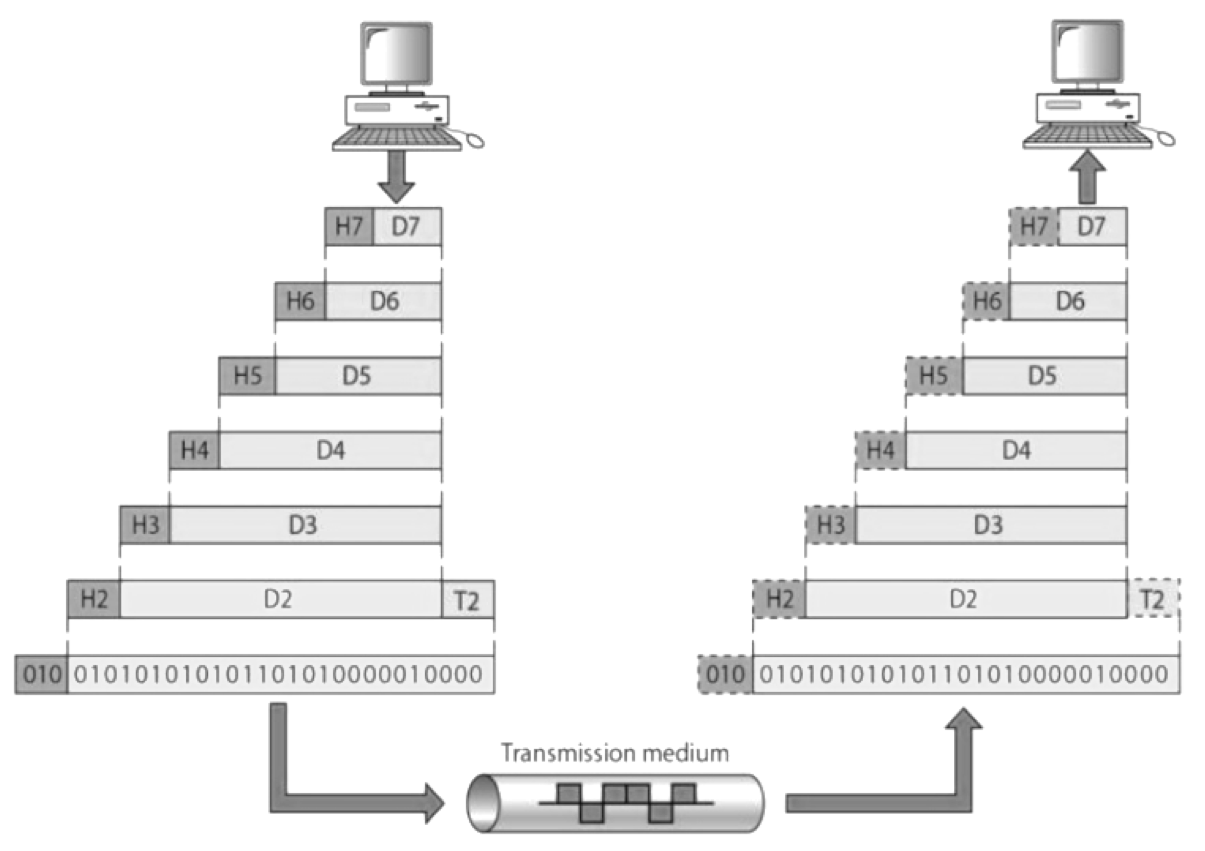
\includegraphics[width=7 cm]{images/OSI-Kapselung}
 \end{minipage}
 
 
 \begin{minipage}[t]{9cm}
 	\textbf{Bit"ubertragung (Physical Layer)}\\
	- "Ubertragung der abstrakten Informationseinheiten '0' und '1' mittels physikalischer Mittel "uber ein Medium.\\
    - "Ubetr"agt einen Bitstrom von Punkt A nach B, ohne dessen Informationsgehalt zu modifizieren. Diese "Ubertragung erfolgt ungesichert, also ohne Fehlertoleranz.
 \end{minipage}
 %
 \begin{minipage}[t]{0.5cm}
 	\-\
 \end{minipage}
 %
 \begin{minipage}[t]{9cm}
 	\textbf{Sicherung (Data Link Layer)}\\
	- Unver"anderte "ubertragen von Daten, d.h. ohne Fehler und in der richtigen Reihenfolge. Sie stellt den "ubergeordneten Schichten gesicherte Verbindungen zur Verf"ugung.\\
	- Durchf"uhrung der Flussregelung, also z.B. die Verhinderung eines Daten"uberlaufs beim Empf"anger (z.B. XON/XOFF-Protokoll).
 \end{minipage}
 
 
 \begin{minipage}[t]{9cm}
 	\textbf{Vermittlung (Network Layer)}\\
	- Verbindet Endsysteme miteinander (z.B. Computer P und Q). Dies kann die Benutzung eines oder mehrerer Kommunikationsnetze einschliessen.\\
	- W"ahlt geeigneten Route (Leitweglenkung, Routing) f"ur das Netzwerk, da meistens verschiedene vorhanden.
\end{minipage}
 %
 \begin{minipage}[t]{0.5cm}
 	\-\
 \end{minipage}
 %
 \begin{minipage}[t]{9cm}
 	\textbf{Transport (Transport Layer)}\\
- Stellt den Anwendungen transparente Datenkan"ale zur Verf"ugung, sie schafft damit Verbindungen zwischen Anwendungsprozessen auf verschiedenen Systemen. Die Transparenz besteht darin, dass von der "ubergeordneten Schicht "ubernommene Daten (Bitstrom) unver"andert "ubertragen werden.
 \end{minipage}

\begin{minipage}[t]{9cm}
 	\textbf{Sitzung (Session Layer)}\\
	- Stellt Mittel f"ur eine geordnete Kommunikationsbeziehung zur Verf"ugung. Dazu geh"ort die Er"offnung, Durchf"uhrung und Beendigung der Session. Jede Session kennt die Phasen Verbindungsaufbau, Datentransfer und Verbindungsabbau.
 \end{minipage}
 %
 \begin{minipage}[t]{0.5cm}
 	\-\
 \end{minipage}
 %
 \begin{minipage}[t]{9cm}
 	\textbf{Darstellung (Presentation Layer)}\\
	- Wird ben"otigt, wenn es um die Beschreibung von Daten geht, sofern diese Beschreibung nicht schon Teil der Applikation selbst ist. Zu diesem Zweck wird die Datenbeschreibung ASN1 (Abstract Syntax Notation One) eingesetzt.
 \end{minipage}
 
 
 \textbf{Anwendung (Application Layer)}\\
"Uber diese Schicht werden den Anwendungen die Kommunikationsdienste in anwendungsunabh"angiger Form zug"anglich gemacht.

\subsection{Allgemeiner Ablauf von Exceptions und Interrupts}
\begin{minipage}{8cm}
Interrupts werden in der Regel von der umgebenen Peripherie oder externen Input-Pins generiert und als Ereignis der CPU-Infrastruktur signalisiert, welche dann eine Handler-Routine einschalten. \\
	\textbf{Siehe} \nameref{Exceptions} Seite: \pageref{Exceptions}
\end{minipage}
%
\begin{minipage}{0.5cm}
	\-\
\end{minipage}
%
\begin{minipage}{10cm}
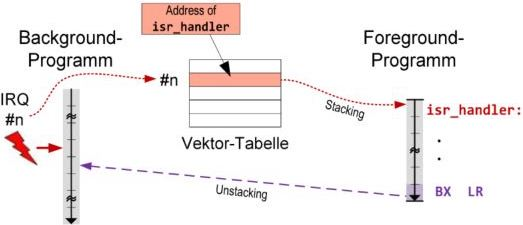
\includegraphics[width=10cm]{images/interruptablauf} 
\end{minipage}

\begin{minipage}{8cm}
	Der allgemeine Ablauf gliedert sich in mehrere Teilschritte:\\
	\begin{enumerate}
		\item Die Peripherie meldet einen Interrupt Request (IRQ) beim Prozessor an
		\item Prozessor beendet die laufende Instruktion (Background)
		\item Prozessor f"uhrt einen Exception Handler oder Interrupt Service Routine (ISR) aus (Foreground)
		\item Prozessor f"ahrt bei der n"achsten Instruktion im Background weiter
	\end{enumerate}
\end{minipage}
%
\begin{minipage}{0.5cm}
	\-\
\end{minipage}
%
\begin{minipage}{10cm}
	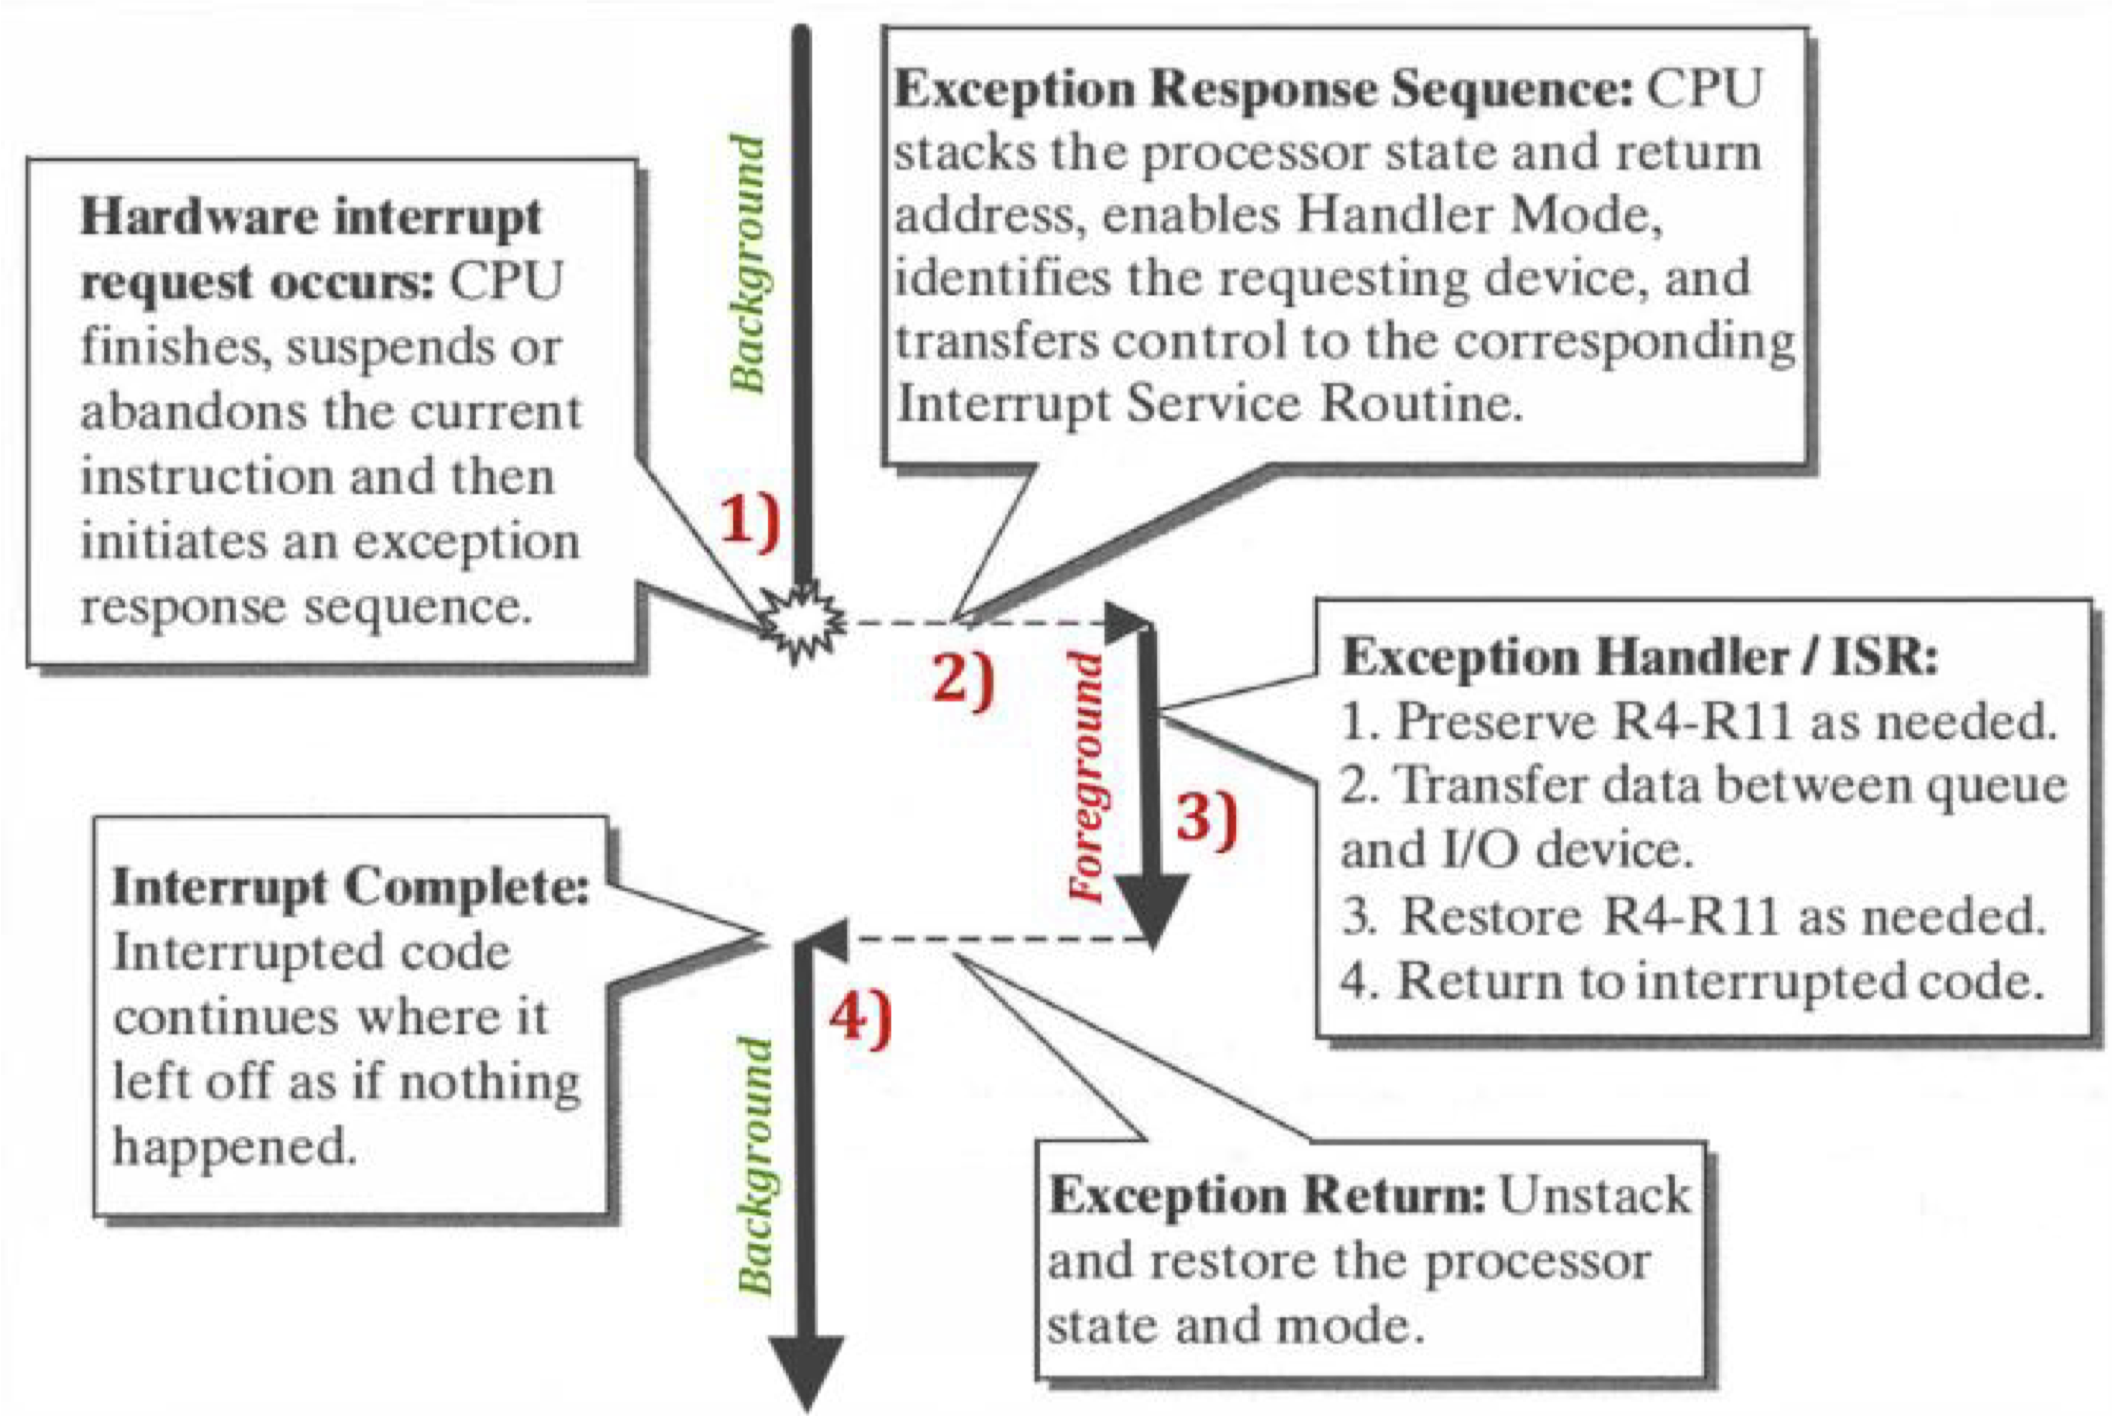
\includegraphics[width=10cm]{images/HW-Interrupt}
\end{minipage}

\subsection{Alternative Ans"atze}
\begin{center}
	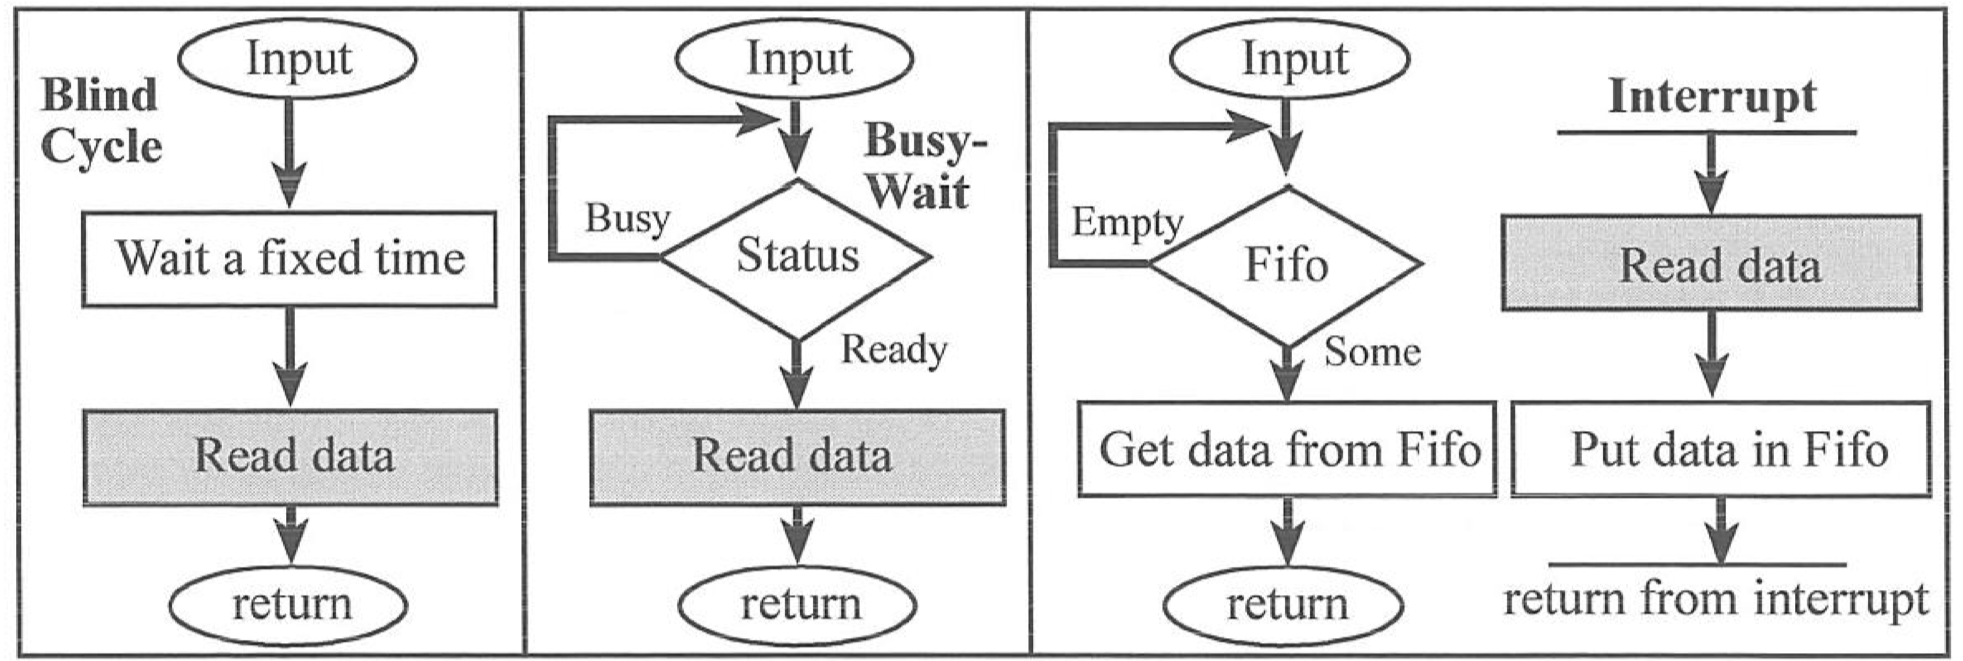
\includegraphics[width=16cm]{images/alternative-lesezugriffe}
\end{center}

\subsubsection{Blind-Cycle}
In der Software wird immer eine fixe Zeit abgewartet, bis die Daten an der
	Hardware abgeholt werden. Diese fixe Blind-Cycle Time ist so zu bemessen, dass die Daten von der HW in jedem Falle bereitgestellt werden k"onnen (worst case scenario).

\subsubsection{Busy-Wait}
In der Software wird solange in einem Loop verweilt, bis die Hardware "uber
eine Status-Information signalisiert, dass die Daten bereitliegen. Damit k"onnen die empfangenen Daten mit Sicherheit abgeholt werden. Es etabliert sich so ein dynamisches Handshaking zwischen der Software und der Hardware.


\subsubsection{Interrupt}
Die Hardware meldet "uber einen IRQ asynchron zum aktuellen
Programmablauf, dass die Daten bereitliegen. Die zugeh"orige ISR unterbricht den
sequenziellen Ablauf im Background-Programm. In der ISR (Foreground) werden die
Daten von der Hardware abgeholt und in einen FIFO-Buffer gelegt. Die Daten k"onnen danach im Background asynchron aus dem FIFO-Buffer gelesen und verarbeitet werden.